%%%%%%%%%%%%%%%%%%%%%%%%%%%%%%%%%%%%%%%%%%%%%%%%%
%%%%%%%%%%%%%%%%%%%%%%%%%%%%%%%%%%%%%%%%%%%%%%%%%

\chapter{Robots}
\label{chap:robots}

%TODO: Introduction. Mention use of artificial robots

\section{Description}

The artificial robots modelled in this study are based on e-puck robots \cite{mondada2009puck}, adapted with grippers. Each robot is equipped with a 360 degree camera to identify objects around them as well as eight local distance sensors spaced equally around the circular perimeter of the robot. Both camera and distance sensors have a depth of view of five times the robot's size. Robots use local communication, which can occur in a radius of five times the robot's size. The sensor and communication range is sufficiently localized. A robot can forage a single item at a time. The robots do not have a global positioning system (GPS) capability to locate items and to position themselves in the environment. As a result robots have to explore the environment to find the prioritized items. Due to the lack of GPS capabilities, robots can not see an item hidden by another item.

Due to the environmental complexity, advanced navigation and obstacle avoidance technique is required. The technique is based on the flocking behaviour of birds used in \cite{antoniou2012congestion}, where robots are pulled to a global attractor, while a local attractor directs robots away from local obstacles but while maintaining a course to the destination. All algorithms use in this paper use the same obstacle avoidance and navigation technique. 

\section{Navigation and Obstacle Avoidance}
\label{robots:obstacleavoidance}

Due to the complexity of the environments, an advanced navigation and obstacle avoidance technique is required.  The technique is based on the flocking behaviour of birds used in \cite{antoniou2012congestion}.

The force that pulls the birds to the destination is known as the global attractor, while a local attractor is a force that directs birds away from local obstacles. As a result birds avoid local obstacles while maintaining course to the destination. 

Figure \ref{fig:obstacleavoidance} illustrates the obstacle avoidance method used by the agents. The obstacle avoidance algorithm achieves the effect of the global attractor by setting the robots field of view towards the direction to the desired destination. The destination is determined by a homing beacon or by the robot's path integration. The direction at the centre of the field of view is the direction to the destination. 

The effect of the local attractor is modelled by evaluating a function for each direction in the field of view, and the most desirable direction is chosen. Desirability, $d$, is defined as a path that achieves an adequate balance between clarity and directness. Clarity id direction $i$, $c_i$, is a normalized proximity sensor or camera reading in the range (0,1) indicating the distance of next nearest obstacle where 0 occurs if no obstacles exist in the destination for the depth of view $v$. The directness of a direction $i$, $\tau_i$, occurs in the range (0,1) and is calculated as the angular deviation from the direction of the destination, where 0 is achieved when the direction $i$ is the same as direction to the destination and 1 occurs when the direction is at the edge of the field of view, $f$. Desirability $d_i$ of direction $i$ is defined mathematically in Equation \ref{eq:1}.

\begin{equation}
	d_i= \lambda c_i + (1 - \lambda)\tau_i \\
	\label{eq:1}
\end{equation} where $\lambda$ determines whether clarity, $c_i$ or directness, $\tau_i$ of direction $i$, has more effect.
 
The described navigation and obstacle avoidance technique is used with all algorithms in the experiment and for algorithms $\lambda$ is set to 0.5.

\begin{figure}
	\centering
	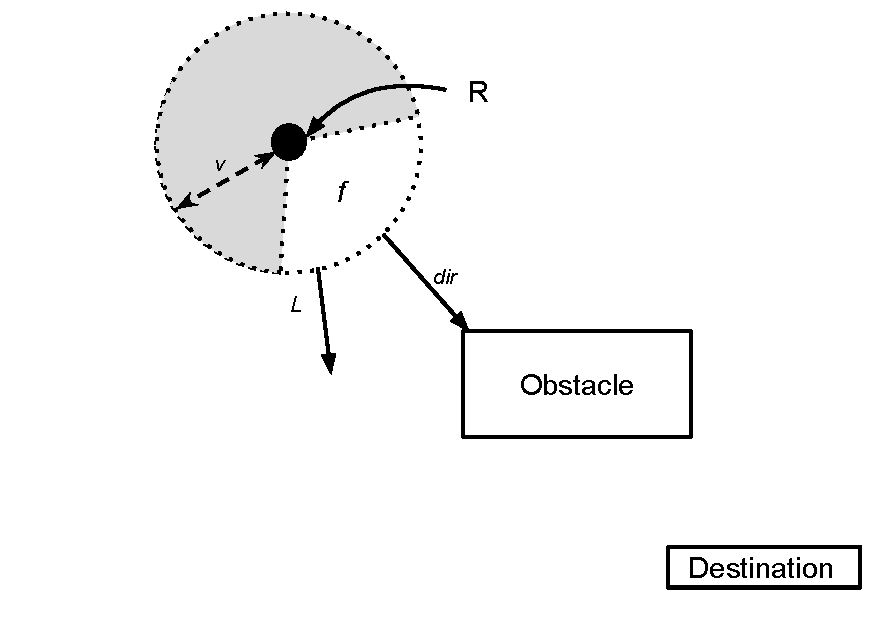
\includegraphics[width=0.5\textwidth]{chapters/chapter5/figures/ObstacleAvoidance.pdf}
	\caption{Obstacle Avoidance. $v$ is depth of view, $f$ is field of view, $R$ is the robot, $dir$ is the direction of the destination, $L$ is a possible value of local attractor}
	\label{fig:obstacleavoidance}
\end{figure}


%%%%%%%%%%%%%%%%%%%%%%%%%%%%%%%%%%%%%%%%%%%%%%%%%
%%%%%%%%%%%%%%%%%%%%%%%%%%%%%%%%%%%%%%%%%%%%%%%%%
\section{Simulator}
A spatially discrete 2-dimensional grid world simulator has been developed and is used for the experimentation in order to accelerate computation \cite{sugawara2002swarming} and also because algorithm performance is sensitive to the amount of time taken to pickup item as well as the manoeuvring capabilities of the robots used \cite{ostergaard2001emergent}. The 2-dimensional grid world simulator allows for movement and pickup time to be standardized across all algorithms for effective comparison. Future studies could include these factors as part of algorithm performance, but are removed for simplification. 

The simulation robots function as follows:
\begin{itemize}
\item Each robot fits into one grid block and each item takes up one grid block. 
\item Only one item or robot can occupy a grid block at a time thus allowing for possible collisions and congestion. 
\item Each robot can only move to an adjacent cell in any direction.
\item Robots can pick up items
\item If a robot does not pick up an item, the item forms an obstacle that must be navigated around
\end{itemize}


The prioritized and non-prioritized sinks were placed next to each other, on a single side of the environment to more accurately represent the type of environment that the problem is most likely to be applied to e.g. in mine tunnels. The sink placement differs from the more common placement at the centre of the environment. The sinks were marked by light beacons that all robots can detect and navigate towards.


%%%%%%%%%%%%%%%%%%%%%%%%%%%%%%%%%%%%%%%%%%%%%%%%%
%%%%%%%%%%%%%%%%%%%%%%%%%%%%%%%%%%%%%%%%%%%%%%%%%
\section{Summary}
\label{robots:summary}

%%%%%%%%%%%%%%%%%%%%%%%%%%%%%%%%%%%%%%%%%%%%%%%%%
%%%%%%%%%%%%%%%%%%%%%%%%%%%%%%%%%%%%%%%%%%%%%%%%%